\chapter{Introduction}\label{chapter_introduction}
\lettrine{R}{eal-time} systems are usually characterized by timely computations, which are bounded by \textit{deadline}, besides correct results of the computations~\cite{Buttazzo2003}. They are applied in many \textit{safety-critical embedded} systems, which are specialized computer systems designed for safety-critical applications~\cite{WangJiacun2017RES}, e.g., the braking system inside vehicles applies proportional force on the wheel to the pressing of a brake pedal in order to slow down (or halt) the vehicle, and must act within sometime otherwise the system fails, consequently, accident can happen. Therefore, safety-critical real-time systems should be analyzed rigorously for functional and timing correctness, which is also specified in the functional safety standards, such as the ISO 26262 ``Road vehicles-Functional safety''~\cite{iso201126262}. The latter standard also suggests the use of \textit{formal methods}, which are mathematical techniques and tools that enable unambiguous specification, modeling and rigorous analysis~\cite{o2017concise}, to develop safety-critical automotive systems.

In distributed computing~\cite{Kopetz2003Real-timeApplications}, the safety-critical software is mapped on multiple hardware systems to capitalize on the computational power provided by the distributed architecture, e.g., the braking software can be executed on multiple electronic control units (ECU). Since the distributed software is  normally exposed to a greater degree of permanent and transient faults, reliability of the safety-critical software should be maximized to improve dependability of the  system which requires additional critical systems resource such as power and energy besides computational resources. However, the embedded hardware is usually resource constrained, therefore, the software should be efficiently mapped to the hardware to conserve critical system resources, thereby accommodate current and future growth of the software functionality.

In this thesis, we apply formal methods to improve the requirements specifications of safety-critical systems, and to analyze the functional and timing behavior of the safety-critical software against the specifications. The safety-critical  specifications should be unambiguous, comprehensible, etc~\cite{ieereqspecstandard}. According to the ISO 26262 standard, semi-formal or formal languages are recommended to specify safety-critical requirements. However, natural language is the de~facto method to specify embedded systems requirements in industry because it is intuitive and expressive, though inherently ambiguous~\cite{ieereqspecstandard}. In the context of natural language, template-based specification and controlled natural language can be considered semi-formal and formal specification methods. The template-based specification methods, e.g., requirements boilerplates~\cite{Hull2011RequirementsEngineering}, property-specification systems~\cite{Dwyer1999PatternsVerificationb}, etc., lack meta-model to effectively create templates, and is usually cumbersome to select the templates. The controlled natural languages, e.g., Attempto~\cite{attempto96}\cite{Fuchs2008AttemptoRepresentation}, etc., renders the syntax and semantics of the natural language and have formal semantics, however lacks support for embedded systems, hence are less effective. In this thesis, we propose a constrained natural language which is domain-specific and uses the notion of boilerplates to facilitate reuse. The specifications have semantics in Boolean logic and description logic to enable rigorous analysis via Boolean satisfiability~\cite{Malik2009BooleanSuccess} and ontology~\cite{f25ea3c6f4b743cd90c150926bbcf3db}, respectively.

The specifications are employed in subsequent system development including software design to verify the latter for correct functionality. The software design is usually modeled, simulated and analyzed before implementation. In this regard, Simulink is one of the most widely used development environment for multi-domain, multi-rate, discrete and continuous safety-critical systems in industry~\cite{JamesB.Dabney2003MasteringSimulink}. For this main reason, there is increasing interest in formal analysis of Simulink models~\cite{Manamcheri2011AModels}. Simulink Design Verifier\footnote{Simulink Design Verifier - https://se.mathworks.com/products/sldesignverifier.html}, which is based on the Prover\footnote{Prover - https://www.prover.com/software-solutions-rail-control/formal-verification/} model checker, is the de~facto tool in the Simulink environment to formally verify Simulink design models. However, it has limited functionality, e.g., it supports only discrete models, has issues with scalability due to state-space explosion, and lacks verification of timed properties~\cite{Leitner2008SimulinkStudy}.  In contrast, we propose a scalable, timed analysis via a statistical model checking~\cite{Legay2010StatisticalOverview}, which uses traces of executions and statistical analysis techniques, e.g., monte-carlo simulation, etc., first by transforming Simulink models into a network of stochastic timed automata using timed-automata patterns~\cite{Filipovikj2018SimppaalModels}.

The software design should be mapped to hardware effectively, that is satisfying the timing and reliability requirements of the distributed safety-critical software, but also efficiently to minimize the power consumption of the distributed system to facilitate extensibility of the software, and also accommodates the demand from the increasing software functionality. We consider the software is scheduled using a fixed-priority preemptive policy, which is quite common in industry, and posses end-to-end timing requirements, e.g., the time duration between the brake-pedal press and the slow-down (or halt) action. Furthermore,  we consider the fault tolerance as a means to maximize reliability of the distribute safety-critical software by mapping redundant software functionality on different computing units.  We propose  \textit{exact} and \textit{heuristic} optimization methods, which deliver optimal and near-optimal solutions, respectively, to efficiently map the distributed safety-critical software to a network of computing units. Specifically, we propose a formulation of integer-linear programming (ILP)~\cite{Mahmud5222}, which is solved using branch and bound. Furthermore, we propose a hybrid-particle optimization~\cite{Mirjalili2019ParticleOptimisation}, which is a meta-heuristic algorithm, to solve the shortcomings of the exact method for large-scale problems~\cite{Mahmud2019Power-awareOptimization} with trade-off over non-optimality.

\section{Research Contributions Overview}
In this subsection, we give overview of the thesis contributions, and later in Section x, the contributions are further discussed in detail.
\begin{itemize}
\item \textbf{Formal Analysis of natural language requirements:}  we propose a fairly expressive, flexible yet structured and domain-specific constrained natural language, called \textit{ReSA}~\cite{resatool}\cite{Mahmud2015ReSA:Systems}. The language has semantics in Boolean and description logic to support for shallow and rigorous analysis, respectively. The Boolean specifications are checked for consistency using the satisfiability-modulo theory via the Z3 SMT solver. Whereas, the description logic is used to encode the specification as ontology, where we check consistency of the specifications at the lexical level using Reasoner (Inference engine) such Hermit. The ReSA tool, which consists of an editor and implements consistency-checking functionality, is integrated seamlessly into EATOP, which is an open source EAST-ADL IDE, to complement the requirements modeling. 

\item \textbf{Scalable analysis of Simulink models:} we propose a pattern-based, execution-order preserving automatic transformation of atomic and composite Simulink blocks into stochastic timed automata that can be formally analyzed using UPPAAL Statistical Model Checker \cite{Bulychev2012UPPAAL-SMC:Automata}. Our method is scalable, and has been validated on industrial use cases \cite{Filipovikj2016SimulinkSystems}. The statistical model checker analyzes a state-transition system by conducting statistical analysis on the collected traces of the system executions, effectively mitigating the state-space explosion of (exact) model checking \cite{Legay2010StatisticalOverview}. 

\item \textbf{Efficient Power consumption ILP and metaheuristics:} we propose an integer-linear programming (ILP) model to the allocation of distributed software on the network of heterogeneous computing units, which have different processor speed, failure rate and power consumption specifications. The ILP implemented in JAVA using the ILOG CPLEX interface, and subsequently solved the CPLEX solver.
\item \textbf{Validation on industrial use cases: } 
Our contributions such as its the ReSA language as well as the proposed formal analysis of Simulink model is validated on industrial use cases, which are provided
\end{itemize}
\begin{figure}
	\centering
	\ifpdf
	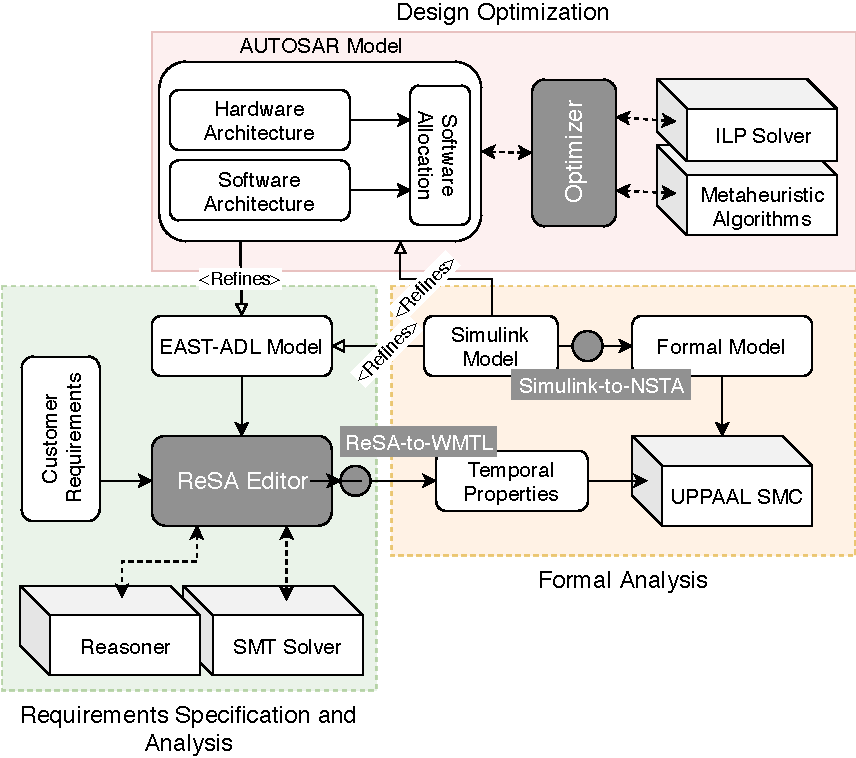
\includegraphics[width=\linewidth]{images/softdevflow}
	\else
	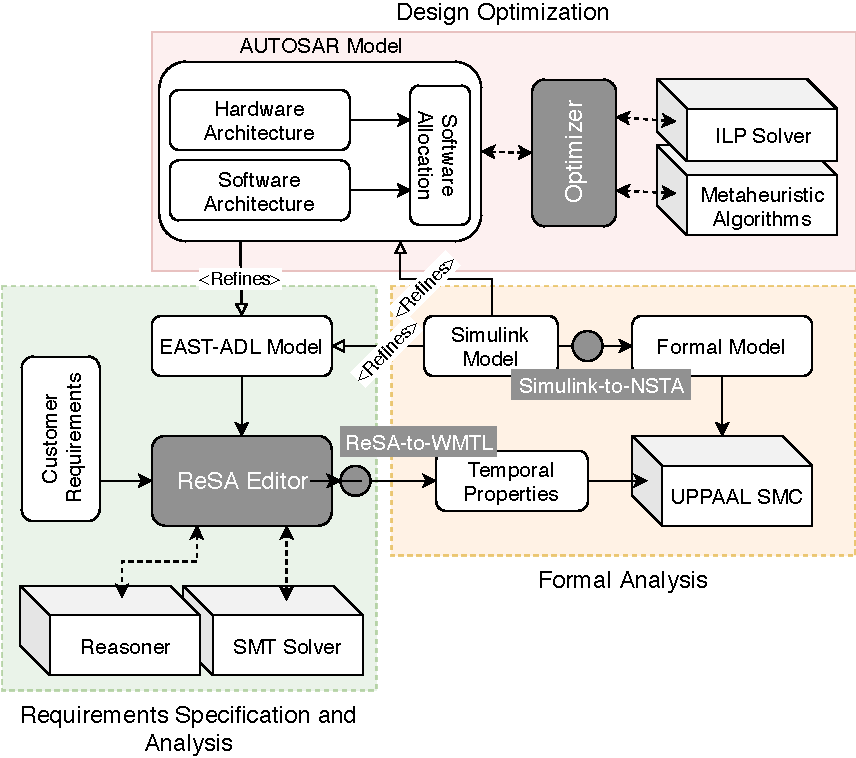
\includegraphics[width=1.0\linewidth]{images/softdevflow.eps}
	\fi
	\caption{Thesis Contributions Workflow.} 
\end{figure}

Our solutions are evaluated on industrial automotive use cases and on a realistic benchmark. The formal analysis of the natural language requirements specifications in ReSA and the formal analysis of Simulink models are evaluated on the adjustable speed-limiter (ASL) and brake-by-wire (BBW) systems provided by Volvo Group Trucks Technology (VGTT). ASL is a speed-limitation automotive function which controls the vehicle speed of Volvo trucks from speeding up, and is useful in roads where speed-limitation signs are in place. The ASL use case consists of around 300 requirements, which are specified in natural language, architectural models in EAST-ADL and Simulink models. The integrated software allocation is evaluated on the engine management system benchmark provided by Bosch~\cite{} provided for AUTOSAR applications. The benchmark consists of statistics of the schedulable objects, such as mean values, shares of timing specifications and activation mechanisms of the schedulable objects in the system.

\section{Thesis Outline Overview}
The thesis is divided into two parts. The first part is a summary of our research. It is organized as follows: in Chapter 2, we give the background information on description logic, Boolean satisfiability problem, Simulink, stochastic timed automata, and meta-heuristic optimization. In Chapter 3, we explain the research problem and outline the research goals. The thesis contributions are discussed in Chapter 4, followed by the related work in Chapter 5. In Chapter 3, we describe the research method applied to conduct the research. Finally, in Chapter 7, we conclude the thesis and outline possible directions for future work.
